\chapter{Methodology \& Theory}
% \addcontentsline{toc}{chapter}{Methodology}
\label{ch:methodology}

This chapter will illustrate the main technologies used in the project. From the web development frameworks, data preprocessing steps, to back-end algorithms, the tools and methodologies that used during the development will be described in detail.


\section{Web Development}

Web is one of the most wide-used networking aids that can fulfil all kinds of user requirements and provide the solution to different problems \cite{lokhande2015efficient}. To develop a well-structured Web application, a suitable technology should be used \cite{lokhande2015efficient}. There are a large number of standard libraries in python that can make web development simple, and Django and Flask frameworks are two popular and frequently-used Web application frameworks. According to \cite{ghimire2020comparative}, Flask is flexible and straightforward controlled, which is easy and quick to learn, while Django is easy to work with because of the substantial libraries and features. 

In this project, the Flask framework in python is chosen to implement the Web application. It provides needed tools, libraries and technologies for back-end development. Flask was developed based on Werkzeug WSGI toolkit, which implements a simple HTTP server and reduces the workload of Web framework development. The structures of Flask can be divided into Static files and Template files \cite{lokhande2015efficient}. The static file contains CSS and JavaScript codes that are the static codes for the website, while the template file has the Jinjia templates for the dynamic page. Additionally, Flask is open-sourced and developers can modify the source code for further design.

In addition, there are many frameworks and libraries for front-end web development, which have helped to promote the development of front-end \cite{dinh2020modern}. In recent years, JavaScript frameworks have made the UI developer more powerful and productive, and React.js, Angular.js and Vue.js are three popular JavaScript front-end frameworks. Vue framework is said to have a high degree of encapsulation and is easy to start because it is simple and reasonable. Vue.js provided data-driven and component-based development by Model View View-Model (MVVM) pattern \cite{li2021research}, which aims to separate the data layer (Model) and UI presentation layer (View), then using ViewModel to achieve the inside logic \cite{anderson2012model}. The following Figure \ref{fig:4} shows the MVVM construction of Vue. Moreover, Vue provides a re-rending feature, because of which most developers prefer to choose Vue.js as the framework \cite{novac2021comparative}. Due to the above advantages, in this project, Vue.js is chosen as the front-end framework for UI development.

 \begin{figure}[H]
    \centering
    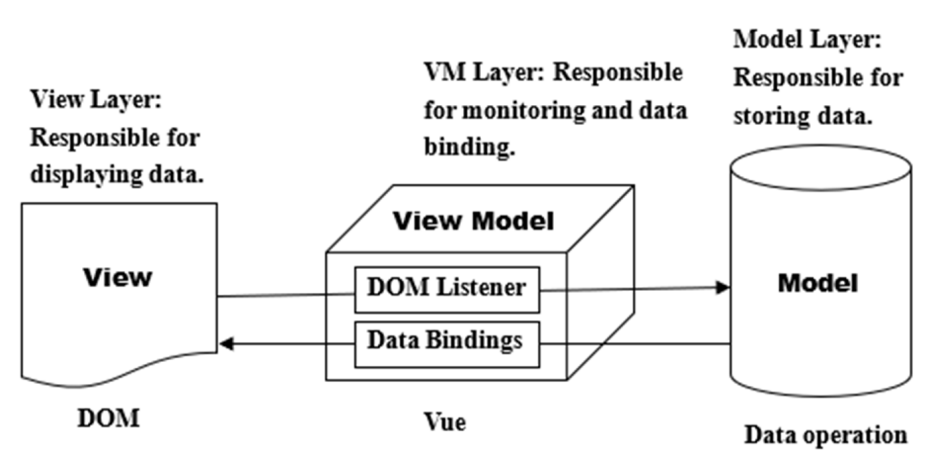
\includegraphics[width=0.6\textwidth]{images/MVVM.png}
    \caption{MVVM Architecture of Vue \cite{li2021research}}
    \label{fig:4}
\end{figure}


\section{CV Parser \& Data Preprocessing}
\label{method_preprocessing}


This section will introduce the technologies for the general parsing processes of unstructured text data and the preprocessing steps in NLP.

The general analysis steps of NLP are shown in Figure \ref{fig:5}, including Lexical Analysis, Syntactic Analysis, Semantic Analysis, Discourse Analysis and Pragmatic Analysis.

 \begin{figure}[H]
    \centering
    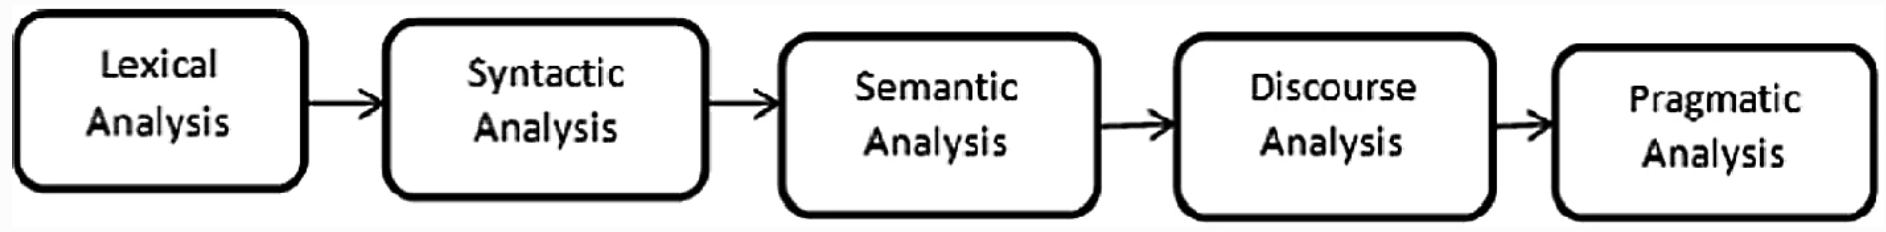
\includegraphics[width=0.8\textwidth]{images/preprocessing_step.png}
    \caption{Analysis Stages in NLP \cite{yogish2018review}}
    \label{fig:5}
\end{figure}

Lexical Analysis is the process that can transform a sequence of characters into tokens \cite{enwiki:1077694767}, which is the first stage of the resume parser. The first phase of the Lexical analyser is scanning, which can divide the input data into syntactic units and categorise them. The second phase is evaluating, which can convert the units into computer-readable values. In our project, the Lexical analyser can be used to parse the input resume to tokens for further processing. As for the second stage of the resume parser, Syntax Analysis takes the input in the form of token streams from the Lexical analyser to parse the code and confirm the rules and the structure of the grammar, then output a parse tree \cite{smith_2022}. A sequence of strings consists of phrases, sentences and paragraphs, and Semantic Analysis is the process related to extracting the structure and language-independent meanings of the sequence. \cite{enwiki:1062314320}. Semantic Analysis can start with the relations between each token to understand the lexical hierarchy such as hyponymy, hypernymy, synonyms and antonyms \cite{manning1999foundations}. In this project, Semantic Analysis can learn the language-independent meanings in the resumes. For example, if the education information from resume A is graduated from 'University of Manchester', and in resume B is 'Manchester University', the Semantic analyser can convert the 'University of Manchester' to 'Manchester University'.

There are many available tools for NLP preprocessing tasks, such as Gensim, NLTK (the Natural Language Toolkit) and Spacy. The comparison of numerous NLP toolkits is shown in Table \ref{tbl:1}. NLTK is a platform to support programs dealing with natural language data, which is regarded as a suitable tool for education, programmers and researchers, and easy to get start with. According to \cite{yogish2018review}, NLTK provides many grammar collections, corpora and trained models for real world data, and comes with many beneficial functions for common NLP tasks. In this project, NLTK is chosen as the toolkit for the data preprocessing tasks.

\begin{table}[htbp]
\centering
\begin{tabular}{|c|c|c|c|c|c|}
\hline
NLP toolkit & Tokenization & POS tagging & Chunking & NER & Stemmer \\
\hline
NLTK & Yes & Yes & Yes & Yes & Yes \\ 
\hline
Apache OpenNLP  & Yes & Yes & Yes & Yes & Yes \\
\hline
Stanford CoreNLP  & Yes & Yes & No & Yes & Yes \\
\hline
Pattern  & Yes & Yes & Yes & No & No \\
\hline
GATE & Yes & Yes & Yes & Yes & No \\
\hline
Spacy  & Yes & Yes & Yes & Yes & No \\
\hline

\end{tabular}
\caption{Comparison of NLP Toolkits \cite{yogish2018review}}
\label{tbl:1}
\end{table}

After parsing the raw text data, the first step is clean the data by removing special characters, carriage returns and line breaks. With the cleaned data, NLP preprocessing tasks could be applied to convenient the subsequent machine learning algorithms. Tokenization is the early step in the NLP pipeline, which is the method that splits the text into tokens. Words, phrases and sentences can all be regarded as tokens, where the word is a token in the sentence and the sentence is a token in the paragraph. NLTK provides several ways to tokenize text. PunktSentence tokenizer can be used to tokenize the text into sentences, and WordPunct tokenizer is based on regular expressions to separate the text by space and punctuation. Additionally, the Treebank tokenizer also uses regular expressions with Penn Treebank corpus to tokenize text, which can separate standard contractions, regard punctuation as the individual token, and split full stops at the end of the sentence. 

Stop word removal is the next widely used method in NLP preprocessing. Words like "the", "a", an "in" occur in all documents frequently and are considered the stop words, which should be removed since they do not contain useful information for further analysis. According to \cite{raulji2016stop}, removing stop words can be applied to strengthen the performance of Information Retrieval System, Text Analytics and Text Summarization tasks. NLTK provides a list of the most common stop word for stop words removal without defining the stop words manually.

 \begin{figure}[H]
    \centering
    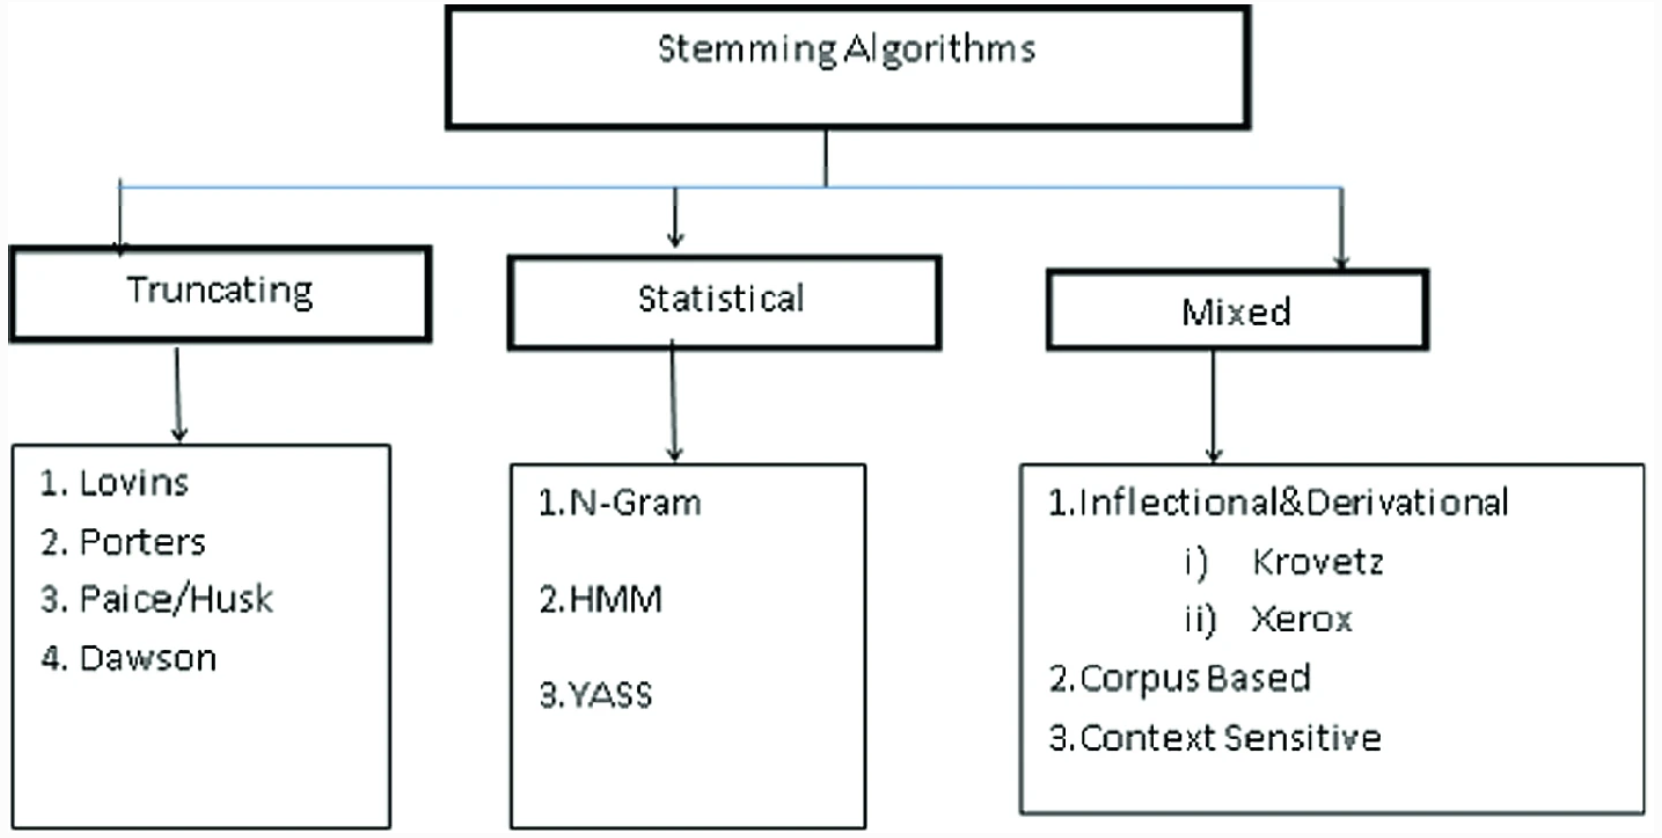
\includegraphics[width=0.9\textwidth]{images/stemming.png}
    \caption{Stemming Algorithms \cite{yogish2018review}}
    \label{fig:6}
\end{figure}

Stemming is a significant preprocessing step that transforms the inflected words to their root form in order to cut down the size of index and increase the accuracy of retrieval. Figure \ref{fig:6} shows the classification of the stemming algorithms. Truncating methods can remove the affixes of the word to build the stem; statistical methods use statistical analysis to produce stem, and stemmers in mixed methods are developed relying on the inflectional and derivational morphology \cite{yogish2018review}. In NLTK, there are several different stemmers such as PorterStemmer, LancasterStemmer and SnowballStemmer. PorterStemmer is one of the most commonly used stemmers, and the output stem is always the short word with the same root meaning.


Lemmatization is the process of gathering the inflected forms of a word so that they can be regarded as a single unit for analysis \cite{enwiki:1100992412}. The lemmatization process is highly close to stemming but includes the intended meaning of a word, which aims to discover the normalized form of the word. For instance, the lemma of the word "better" is "good". NLTK contains the method WordNetLemmatizer() to lemmatize a word by its context and usage in the sentence, which can be used for text understanding, clustering, tokenization and visualization. 

Part of Speech (POS) labelling is another vital preprocessing method that assigns the part of speech tags for each word in a sentence, where POS is a kind of grammatical feature including nouns, verbs, adjectives, et cetera. According to \cite{kumawat2015pos}, POS tagging is known as a necessary tool for numerous NLP activities, like word disambiguation, information recovery, and machine interpretation. The following Figure \ref{fig:7} shows the process of POS tagging, where the tagging algorithm allocates the tags to individual tokens and compares them with the tag set. There are rule-based, stochastic, and hybrid approaches for POS tagging. Rule-based tagger searches the dictionary and returns all the possible tags, then removes ambiguous words using the linguistic features by hand-coded rules to get the single POS tag of a word \cite{yogish2018review}. In contrast, the stochastic tagger assigns the tags by probability and statistics based on corpus evidence. The hybrid approach combines the rule-based and statistical methodology together \cite{rathod2015survey}, which uses hand-coded rules to illustrate the tags and applies statistical machine learning methods to induce rules from the training corpus. NLTK POS tagger uses the Penn Treebank tag set as default and the maximum entropy model to generate the tagged corpus.

 \begin{figure}[H]
    \centering
    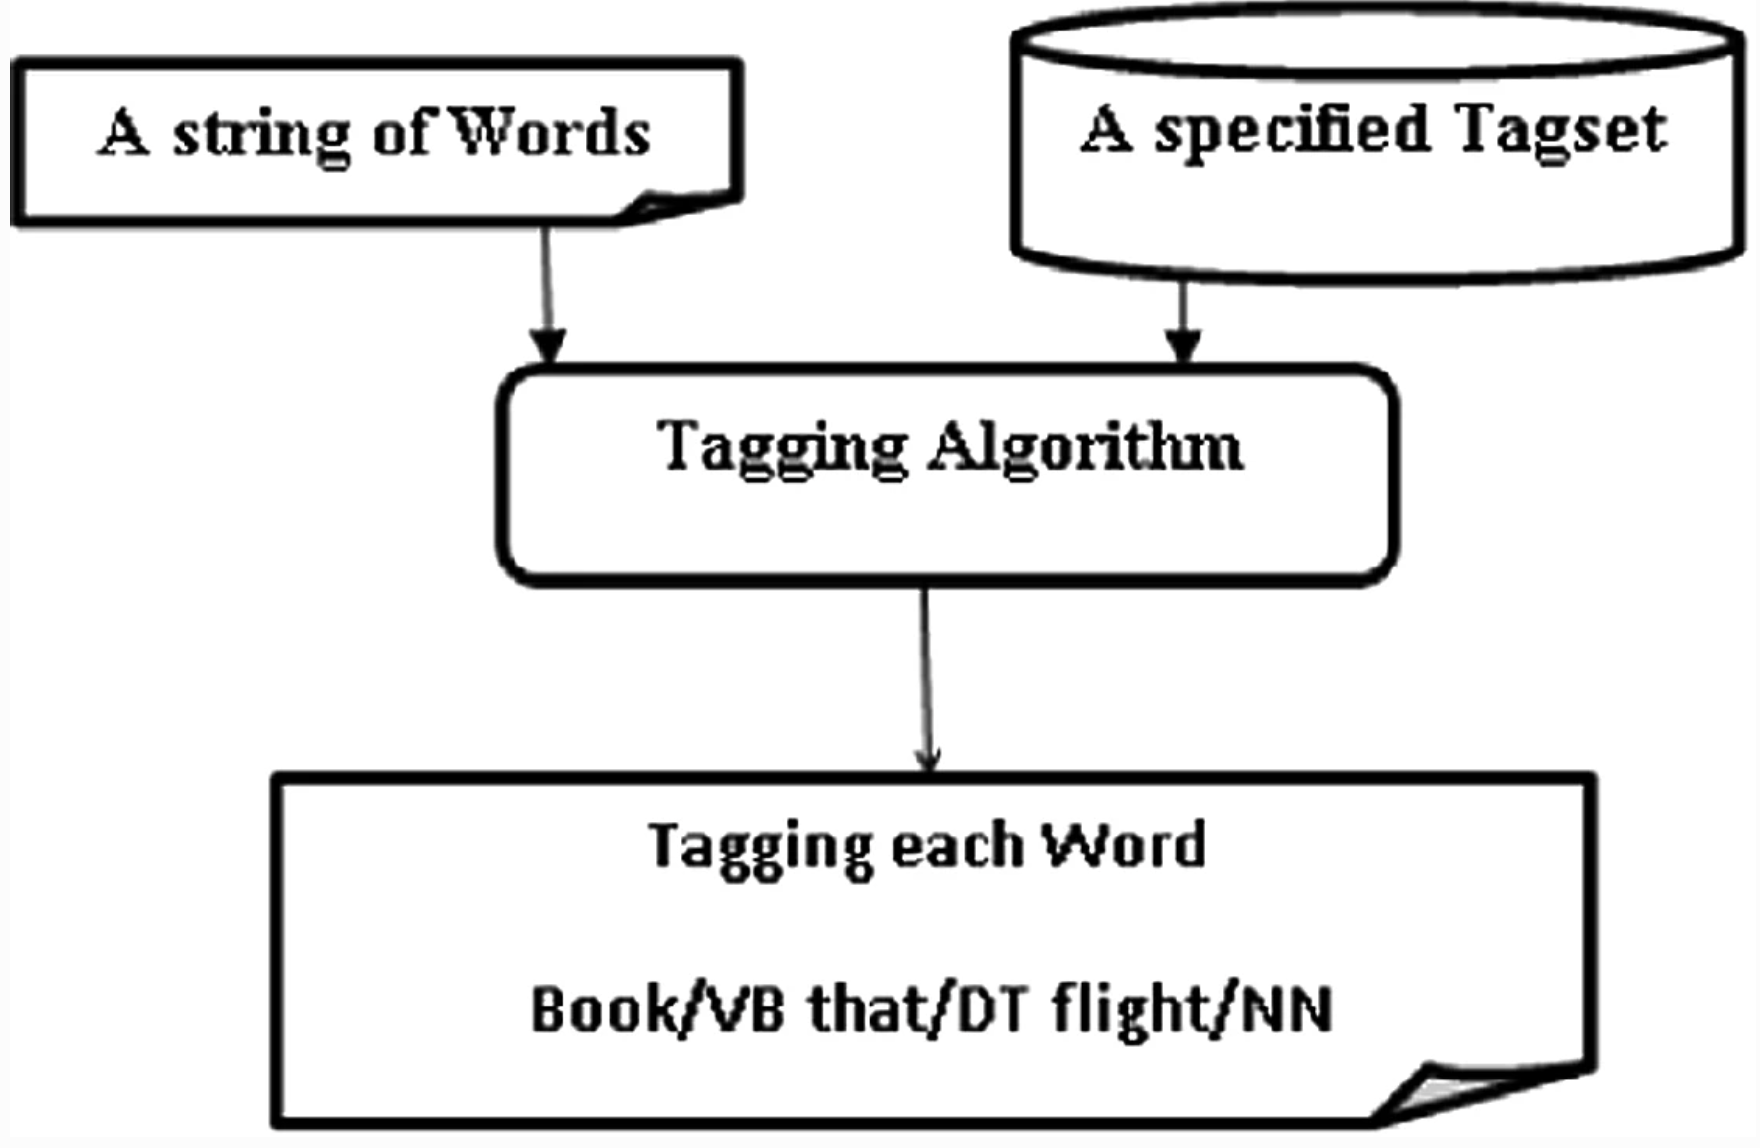
\includegraphics[width=0.5\textwidth]{images/POS.png}
    \caption{Process of POS Tagging \cite{yogish2018review}}
    \label{fig:7}
\end{figure}



\section{Related Techniques}
As illustrated in Chapter \ref{ch:background}, NLP and machine learning techniques would be used to achieve the resume-checking function. This section will describe the methods and tools related to the back-end algorithms separately, including information recognition, skill extraction, and skill matching.

\subsection{Information Recognition}
% NER / profile info / skill extraction (clustering, topic modeling, Bert)
% word embedding

Checking the integrity of personal information in the resume is one of the main tasks for this CV checker, which means the information such as name, e-mail address, education and work experience should be recognized by the back-end algorithms. Named Entity Recognition (NER) can be used as the tool for this task.


NER can implement the information extraction task by locating and classifying real-world objects or proper nouns in unstructured text data. Pre-defined categories such as organizations, locations and persons can be recognized in the text data by NER, and many applications like Information Retrieval System \cite{khalid2008impact} have been improved on account of the usage of NER. According to \cite{mohit2014named}, there are two sub problems of NER, one is named entity boundaries' recognition, and the other is the categories recognition. Dictionary-based, rule-based and machine learning-based are the three approaches of NER. The dictionary-based approach can match features by dictionary looking up, which is a simple method and can obtain good precision. Nevertheless, this hand-crafted-based system requires a massive effort by domain experts to build the dictionaries and is said to have difficulty in complete coverage for many named entity categories \cite{neelakantan2015learning}. The rule-based method uses rules and patterns of named entities which can consider the context of the entities, but the rules should be written before recognition. For this project, the information that needs to be extracted is personal information instead of proper nouns. Therefore, the dictionary-based and rule-based approaches are unsuitable since it is hard to write the common rule set for the entities.

Machine learning-based methods utilize statistical models to recognize the named entities in the text. Hidden Markov Models (HMMs), Conditional Random Fields (CRFs) and Neural Network models can be applied to the NER problem. CRFs is a discriminative sequence framework for sequence labelling, which aims to find the most probable label sequence $y^*$ given the observation sequence $x$ \cite{lafferty2001conditional}, 

\begin{equation}
    y^* = \mathop{\arg\max}{_yp(y|x)}
\end{equation}

where $x$ consists of the sequence of the input tokens. The computation of probability is as follows, where $w$ refers to the weight, $f$ is for the feature function, $T$ refers to the summation of all tokens and $K$ means the summation over all feature functions \cite{lafferty2001conditional}:

\begin{equation}
    p(y|x) = \frac{1}{Z_x}\exp(\sum_{t=1}^{T}\sum_{k=1}^{K}w_kf_k(y_t,y_{t-1},x_t))
\end{equation}

CRFs models can be approximately interpretable and do not need pre-trained vectors. However, it performs prediction using input features, which means feature engineering should be completed before training. Neural networks can handle the sequence processing problem without feature functions, which can detect implicit features from the input data automatically by hidden layers. Take BiLSTM as an example, the feature function in CRFs can be replaced by:

\begin{equation}
    f(tag_i, tag_{i-1}, token_i) = Wh_i + b
\end{equation}

In this project, spaCy is used for the NER task, which is an application-oriented, open-sourced library for NLP. SpaCy supports deep learning workflows, allowing its deep learning library Thinc to connect statistical models trained by other machine learning libraries such as TensorFlow \cite{enwiki:1094217869}. Thinc is a lightweight deep learning library powering spaCy, with which, as the back-end, Convolutional Neural Network (CNN) models can be applied in spaCy to advanced NLP tasks such as POS tagging and NER. With spaCy, developers do not need to take time to build or adjust the neural network structure because spaCy provides the most advanced neural network framework for NER model training instead. According to the official document of spaCy \cite{honnibal_2022}, the NER system presents a highly-developed word embedding approach. It uses the features of subword and Bloom embedding, a Convolutional Neural Network with residual connections, and a transition-based method for named entity parsing, where bloom embedding is an approach that can reduce the model size of NER. This system is developed to balance the efficiency, accuracy and flexibility of NER model training. With a normalized training dataset containing named entity tags, the spaCy NER model can be trained and used to recognize the pre-defined named entities in the new input data.

\subsection{Skill Extraction}

Extracting skills from the resume and the job description data is another main task for the back-end algorithm. NER can also be utilized for skill extraction if suitable training data exists with named entity labels. Otherwise, techniques like clustering algorithms, topic modeling and Bidirectional Encoder Representations from Transformers (BERT) could be considered utilized for the skill extraction task from text data.


The basic idea of using clustering algorithms to extract skills in a document is regarding the word vectors as the samples and gathering them into different groups, which are expected to have one or more clusters indicating to different kinds of skills. 

\subsubsection{Word Embedding \& K-means Clustering}
\label{sec:word2vec}

Before clustering, word embedding techniques should be used for the representation of words in the form of vectors. Word2vec is an approach that can learn the correlation among words from the corpus by neural network and represent each word as a vector. Based on a word's usage in the text, word2vec can infer the meaning of the word with a high level of accuracy. The output is vectors for each word with remarkable linear relationships, which can be calculated like \cite{mikolov2013efficient}:

\begin{equation}
    vec("king") - vec("man") + vec("woman") =~ vec("queen")
\end{equation}

The assumption to get the words' representation is: 1) there is a vector $v \in R^d$ to represent each word $w \in V$; 2) there is a probability $Pr(w|u_1,u_2,...,u_l)$ for the word $w$ appears in a context $(u_1,u_2,...,u_l)$. The task is to find the vector $v$ that can maximize the probabilities for each word $w$ and the context $(u_1, u_2,...,u_l)$, where neural network parameters can be used to compute the probabilities by minimizing the cross-entropy loss.

Continuous bag-of-words (CBOW) and Skip-gram architectures are utilized in Word2vec to generate the distributed word vectors. CBOW model predicts a word from the surrounding words with the architecture shown in below Figure \ref{fig:8}:

 \begin{figure}[H]
    \centering
    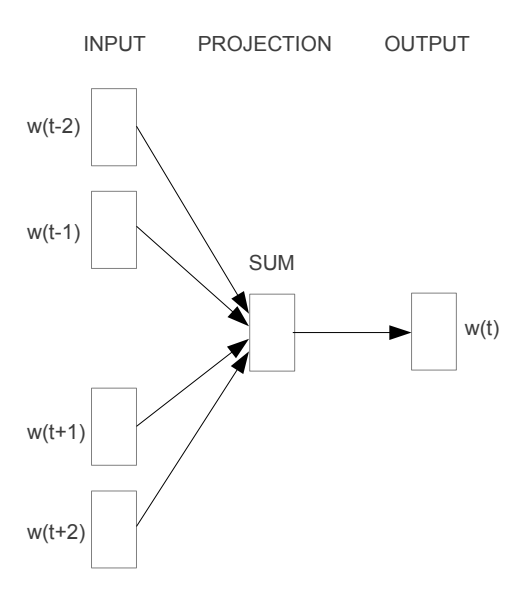
\includegraphics[width=0.35\textwidth]{images/CBOW.png}
    \caption{Model Architecture of CBOW \cite{mikolov2013efficient}}
    \label{fig:8}
\end{figure}

where the probability $Pr$ of word $w_t$ appears in its context $(w_{t-1},...,w_{t-m+1})$ is:

\begin{equation}
    Pr(w_t|w_{t-1},...,w_{t-m+1}) = softmax(Wy)
\end{equation}

\begin{equation}
    y = average(w_{t-1},...,w_{t-m},w_{t+1},...,w_{t+m})
\end{equation}

In contrast, Skip-gram uses a neural network model to predict contextual words instead of a target word, and the structure of the model is shown in the following Figure \ref{fig:9}. According to \cite{mikolov2013efficient}, Skip-gram performs well with a small amount of data and is effective at representing uncommon words, while CBOW is faster and more suitable for representing frequent words.

 \begin{figure}[H]
    \centering
    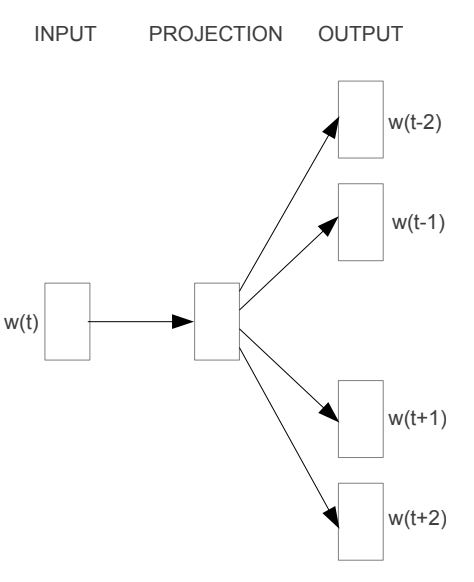
\includegraphics[width=0.35\textwidth]{images/skip_gram.png}
    \caption{Model Architecture of Skip-gram \cite{mikolov2013efficient}}
    \label{fig:9}
\end{figure}

Word2vec algorithm can be implemented by Gensim, an open-sourced library contains word2vec algorithm, latent semantic analysis and so on. Moreover, Gensim provides both CBOW and Skip-gram algorithms to train the model and get the word vectors. In this project, Gensim would be used as the tool to get the representation of the words for the subsequent clustering algorithm.

After getting the word embeddings, K-means algorithm can be used to partition the word vectors as the samples to get the expected skill clusters. K-means algorithm assumes that a given sample set could be separated into K clusters based on the distance between the samples and the centers \cite{macqueen1967classification}. The distance among the clusters is anticipated to be sufficient and the member points in each cluster are expected to be as close as possible to one another. Scikit-learn, a progressively popular machine learning library, provides the implementation of K-means algorithm, which will be used in this project to get meaningful clusters. With the trained clusters, each word in a new input document can be allocated to a suitable cluster, where those assigned to skill clusters are identified as skills in the text.


\subsubsection{Topic Modeling}
%Topic modeling
Besides K-means clustering algorithm combined with word embedding techniques, topic modeling is also a clustering tool for figure out the connection among text content. The skill vocabularies or phrases can be regarded as keywords in the job description. Topic Modeling techniques are expected to extract the important keywords by treating words in the corpus as features.


Unlike K-means, topic modeling is a probability-based algorithm using an unsupervised machine learning approach to identify word clusters through a set of documents. Latent Dirichlet Allocation (LDA) model is a classic topic model with a three-level hierarchical Bayesian model proposed by Blei et al. \cite{blei2003latent}, which applies Dirichlet distribution as the prior and estimates the posterior to infer the parameters by learning from the given document set. LDA assumes that each document is generated by potential topics and each topic is a probabilistic distribution over words. The graphical representation of LDA is as following Figure \ref{fig:10}, where $\alpha$ and $\beta$ are given parameters, $\theta$ is the joint distribution of a topic mixture, inner rectangle $N$ denotes the replicates of the selection of topics $z$ and words $w$ in a document, and outer rectangle $M$ represents the repeats of the document generation process \cite{blei2003latent}. And the purpose of LDA algorithm is to extract the latent topics in a set of the document by determining the probability that a word is associated with a topic and the proportion of a document that is related to a topic.

 \begin{figure}[H]
    \centering
    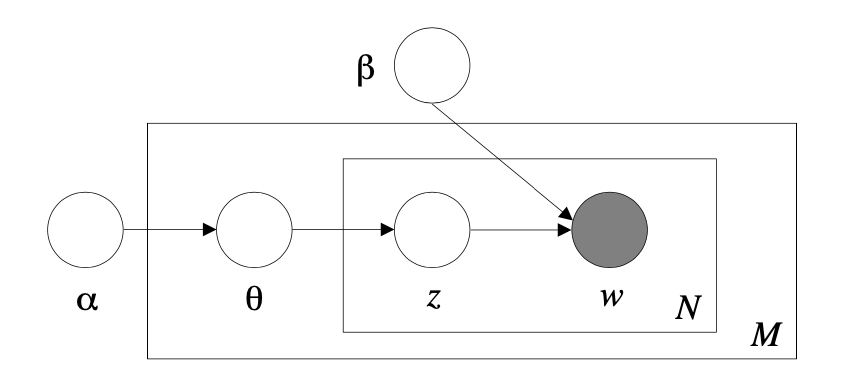
\includegraphics[width=0.5\textwidth]{images/LDA.png}
    \caption{Graphical Representation of LDA \cite{blei2003latent}}
    \label{fig:10}
\end{figure}

Gensim provides an optimized LDA implementation, which not only enables estimating the LDA model from the training corpus, but also can infer the topic distribution on new documents. The output topics are represented by the combination of top keywords in each topic with their weight. Additionally, the Gensim LDA module provides the perplexity and coherence score for the topic to evaluate the generated topic model. 

\subsubsection{Hybrid Approach}
\label{sec:hybrid}

Without a sufficient skill database, Some simple approaches might not produce the desired extraction result. In this situation, combining several NLP techniques and a machine learning-based classifier may perform better. Ketterer \cite{ketterer} proposed an approach that used POS, Chunking and a BERT Embedding classifier to identify the skills in the job description. The overall design of this hybrid approach is depicted in Figure \ref{fig:13}, where the regex (regular expression) chunking strategy is used to obtain the potential phrases, and the training set of the subsequent neural network is made up of the labeled extracted chunks.

 \begin{figure}[H]
    \centering
    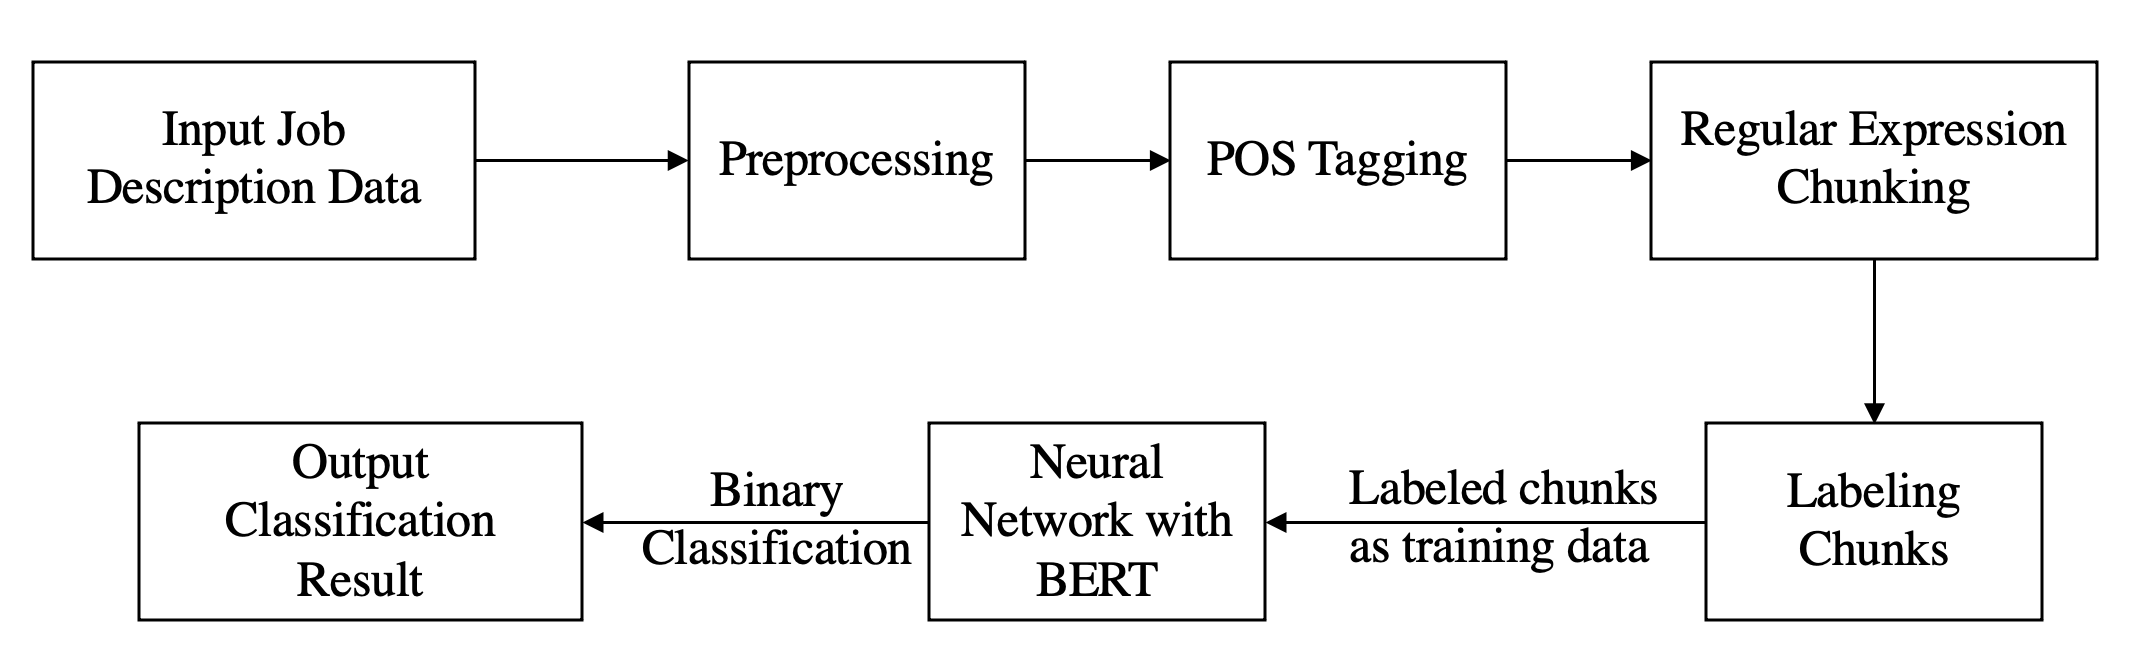
\includegraphics[width=0.85\textwidth]{images/Process.png}
    \caption{Overall Process}
    \label{fig:13}
\end{figure}


Preprocessing techniques and POS tagging are introduced in the previous sections, which are the first two steps in this model. Given the job description data, clean the dataset by tokenization, stemming, removing stop words and other preprocessing methods, then identify the Part of Speech in each job description for further analysis. 

POS tagger labels the individual words in the text with their probable Part of Speech. To understand the structure of the text and extract the patterns that might contain the skill expressions, Chunking should be used to determine certain phrases according to the words' POS combinations. The chunking algorithm takes POS tags as the input and outputs the chunks in the text. According to \cite{d'souza_2018}, Chunking is crucial when extracting Location, Organization, and Person Name information from the text. Similar to POS tag sets such as Penn Treebank tagset, phrase tags also have standard types like Noun Phrase(NP), Preposition Phrase(PP), etc. For the chunking process, NLTK provides a technique for the generation of chunks with the use of regular expressions. Ketterer defined four patterns' regular expressions for the phrases might hold the skill terms: Noun Phrase, Noun Phrase with preposition or conjunctions, Verb Phrase and Nouns between commas \cite{ketterer}. With these regular expressions, NLTK can extract the potential skill phrases to build the training dataset.

The extracted phrases are labeled to 1 (isSkill) or 0 (notSkill) manually, and a neural network are built to handle the binary classification of phrase samples. Transfer learning is a machine learning research subject that concentrates on storing knowledge obtained from one task and applies to the other related task \cite{enwiki:1099727359}, which means the pre-trained model can be regarded as a start point for a new model on different problem. Therefore, transfer learning enables the training process to depend less on the volume of data and results in better learning performance than training on a small dataset alone \cite{zhuang2020comprehensive}. Bidirectional Encoder Representations from Transformers (BERT) is a state of the art NLP model, which has been pre-trained by numerous corpora to produce better word embedding. With the advantage of word embeddings, BERT is used in this skill extraction task to generate significant robust, contextual understanding and semantic similarity word embeddings \cite{ketterer2}. The structure of the BERT layer is as follows.

 \begin{figure}[H]
    \centering
    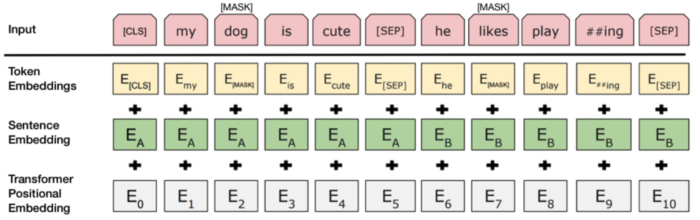
\includegraphics[width=0.85\textwidth]{images/BERT.png}
    \caption{Structure of BERT Layer \cite{ketterer2}}
    \label{fig:11}
\end{figure}

% Using the BERT layer, the architecture of the neural network is shown in following Figure \ref{fig:12}.

%  \begin{figure}[H]
%     \centering
%     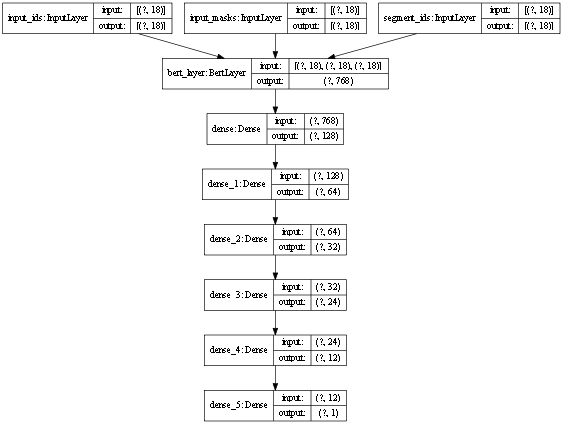
\includegraphics[width=0.9\textwidth]{images/withBERT.png}
%     \caption{Architecture of Neural Network \cite{ketterer2}}
%     \label{fig:12}
% \end{figure}

The trained neural network model enables to determine whether the phrase is a skill or not. When inputting an unseen job description, the text should be preprocessed, labeled with the POS tags and chunked. Then the neural network model with BERT layer is utilized to determine the skills in the extracted chunks.


\subsection{Skill Matching}

The match rate between resume and job description could be calculated using the extracted skills from both the two text, because in this project, skill matching is the most concerning part.

A straightforward idea to calculate the match rate is using semantic cosine similarity. Cosine similarity is measured by the cosine value of the angle between the text vectors to detect if they are pointing to a similar direction \cite{han2011data}, where larger cosine values denote smaller vectors' angles. Word embedding techniques like Word2Vec and TF-IDF (Term Frequency-Inverse Document Frequency) can convert the process from linguistic sentences to vectors. Word2Vec algorithm has been introduced in the previous Section \ref{sec:word2vec}, which is a prediction-based approach for word embedding, while TF-IDF is a count-based approach. The aim of TF-IDF is to emphasise terms that only appear in a few documents while weighing down the common words that are used in almost all documents. TF is the term frequency of a word, which means the count of the word appearing in one document, and IDF denotes the inverse document frequency, whose value would be smaller if the words occurred in the corpus frequently. The formulas for word $i$ in document $j$ are as follows:

\begin{equation}
    {TF_{i,\ j}=\ \frac{n_{i,j}}{\sum_{k}n_{k,j}}}
\end{equation}

\begin{equation}
    IDF_i=\log{\frac{|D|}{\{j\ :\ t_i\ \in d_j\}\ +\ 1}}
\end{equation}

where $n_{i,j}$ represents the count of word $i$ in the document $j$, $\sum_k n_{k,j}$ denotes the sum of the count of the words' occurrence in document $j$, $|D|$ is the number of all documents and $\{j\ :\ t_i\ \in d_j\}$ means the count of documents taht contain word $i$. And $TF - IDF$ of word $i$ in document $j$ is calculated by the product of $TF_{i,j}$ and $IDF_{i,j}$.

Based on the two vectors generated from embedding techniques, the cosine similarity can be computed by the following formula:


\begin{equation}
    cos(\theta) = \frac{\sum_{i=1}^{n}(x_i \times y_i)}{\sqrt{\sum_{i=1}^{n}(x_i)^2} \times \sqrt{\sum_{i=1}^{n}(y_i)^2}}
\end{equation}

Further on, apart from getting the match rate, the CV checker is expected to check the single skill matching, which means each skill extracted from the job description needs to be checked in the resume. The simplest method is using a pattern matching algorithm to check if the exact skill tokens are present in the resume sequence. Nevertheless, because of the diversity of natural language, the pattern matching approach might not get the expected match result since one skill could have multiple expressions in terms of numerous stem forms. For instance, "software development" and "develop software" should be regarded as the same skill but not the exact same pattern. 

In this case, the skill match process should take some 'tolerance' into account, which means the two skills do not need to be exactly the same pattern but still can be viewed to express the same skill. For each skill in the job description, we traverse all the skills in the resume to find the most matching skill by calculating the cosine similarity. Additionally, a threshold for the cosine similarity value should be set to determine whether this most similar expression presents the same skill as the target one.
